% FOSS4G 2026: Natural-Language Routing on an Open Stack.
% Default Beamer theme. Build: tectonic talk.tex (screenshots from ../screenshots, made by
% scripts/capture_talk.py). Speaker notes for every slide: ../README.md.
\documentclass[aspectratio=169]{beamer}
\setbeamertemplate{navigation symbols}{}
\setbeamertemplate{footline}[frame number]
\usepackage{amsmath,amssymb}
\usepackage{graphicx}
\graphicspath{{../screenshots/}}

\newcommand{\shot}[1]{\includegraphics[width=\linewidth]{#1}}
\newcommand{\api}[1]{\texttt{#1}}

\title{Natural-Language Routing on an Open Stack}
\subtitle{Language becomes constraints; constraints become geometry}
\author{John Gunnar Carlsson \and Andreas Royset}
\date{FOSS4G 2026 \\ Wednesday, November 4, 15:00 \\ Compagno}

\begin{document}

\begin{frame}
  \titlepage
\end{frame}

% ------------------------------------------------------------------------------------------------
\section{Approach}

\begin{frame}{Maps expose toggles; requests are constraints}
  \begin{itemize}
    \item What navigation products accept:
      \begin{itemize}
        \item global switches: avoid highways, tolls, ferries
        \item search ranked by distance from the user (``coffee near me'')
      \end{itemize}
    \item What people actually ask for:
      \begin{itemize}
        \item ``gas on the right, so I don't turn across traffic''
        \item ``coffee about an hour from now''
        \item ``stay off 880''
        \item ``between the two of us, who picks up our daughter?''
      \end{itemize}
    \item Each is a constraint expressible in plain language and computable with open tools
  \end{itemize}
\end{frame}

\begin{frame}[fragile]{Approach: the model fills in a form}
  \begin{columns}[T]
    \begin{column}{0.48\textwidth}
      \begin{itemize}
        \item Language $\to$ typed constraint object (JSON schema, structured output)
        \item Constraints $\to$ geometry and solver input, by deterministic code
        \item The model never routes, searches, or optimizes
        \item No coordinates, no store names; no start: \texttt{origin: null} is the phone's GPS
        \item Every result is re-checked against the final route
      \end{itemize}
    \end{column}
    \begin{column}{0.48\textwidth}
\begin{semiverbatim}\scriptsize
\{
  "origin": null,
  "destination": "home",
  "stops": [
    \{"kind": "errand", "what": "pharmacy",
     "closesAt": "18:00"\},
    \{"kind": "errand", "what": "groceries"\},
    \{"kind": "errand", "what": "gas"\}
  ],
  "stopOrder": "any",
  "arriveBy": "18:15"
\}
\end{semiverbatim}
      {\footnotesize ``I need a pharmacy before it closes at six, groceries, and gas, in any order, and I have to be home by 6:15.''}
    \end{column}
  \end{columns}
\end{frame}

\begin{frame}{Tools}
  \begin{itemize}
    \item Valhalla (OpenStreetMap graph): \api{/route}, \api{/sources\_to\_targets}, \api{/trace\_attributes}, \api{exclude\_locations}, time-dependent costing
    \item Overture Maps places (GeoParquet, 273k in the Bay Area), queried in place with DuckDB
    \item Photon and Nominatim: OSM geocoding, self-hosted
    \item OR-Tools routing: disjunctions, time windows, pickup and delivery
    \item Language model behind a JSON schema: Ollama locally, or any OpenAI-compatible API
    \item Caltrans PeMS loop detectors: hour-of-week speeds loaded as Valhalla predicted traffic
    \item Ferrostar (Rust $\to$ WebAssembly): turn-by-turn in the browser
    \item One laptop, 12 GB GPU; all five demos also run on a local qwen3.6 35B-A3B (18--61 s each)
  \end{itemize}
\end{frame}

% ------------------------------------------------------------------------------------------------
\section{Five requests}

\begin{frame}{Five requests from the Great Mall, Milpitas}
  \begin{itemize}
    \item Start: a GPS fix posted by the phone; no request states where the driver is
    \item Requests, and what each exercises:
      \begin{enumerate}
        \item Gas on the right, on the way to Levi's Stadium \\ \quad {\small DuckDB on Overture; arrival-side geometry}
        \item Coffee about an hour into the drive to Sacramento \\ \quad {\small maneuver times; Valhalla matrix}
        \item Oakland airport, but stay off 880 \\ \quad {\small map-match, exclude, re-route}
        \item Pharmacy before 6, groceries, gas, home by 6:15 \\ \quad {\small OR-Tools: disjunctions and time windows}
        \item Split the afternoon's tasks between two drivers \\ \quad {\small OR-Tools: two vehicles, pickup and delivery}
      \end{enumerate}
    \item All screenshots come from the live path (model in the loop), via \texttt{scripts/capture\_talk.py}
  \end{itemize}
\end{frame}

\begin{frame}{1. Gas on the right}
  \begin{columns}[T]
    \begin{column}{0.4\textwidth}
      {\small
      \textbf{Prompt}

      ``Take me to Levi's Stadium, and get gas on the way at a station on the right so I don't have to turn across traffic.''

      \medskip
      \textbf{Result}

      The route stops at a 76 station on West Calaveras Boulevard. The station is on the right when the driver arrives, and the stop adds about 30 seconds.
      }
    \end{column}
    \begin{column}{0.58\textwidth}
      \shot{gm-gas-right.png}
    \end{column}
  \end{columns}
\end{frame}

\begin{frame}{2. Coffee during the drive}
  \begin{columns}[T]
    \begin{column}{0.4\textwidth}
      {\small
      \textbf{Prompt}

      ``I'm driving to the Sheraton in downtown Sacramento, and I'm going to want coffee about an hour from now. Keep the detour small.''

      \medskip
      \textbf{Result}

      There was no coffee shop near the exact one-hour point, so the app widened the search slightly and said so. It chose a Peet's in Pleasant Hill, reached about 50 minutes into the trip, with a detour of about 20 seconds.
      }
    \end{column}
    \begin{column}{0.58\textwidth}
      \shot{gm-coffee-hour.png}
    \end{column}
  \end{columns}
\end{frame}

\begin{frame}{3. A route that avoids I-880}
  \begin{columns}[T]
    \begin{column}{0.4\textwidth}
      {\small
      \textbf{Prompt}

      ``Get me to Oakland airport, but stay off 880.''

      \medskip
      \textbf{Result}

      The route takes I-680 and I-580 instead of I-880. It takes 63 minutes, about 20 minutes longer than the usual route.
      }
    \end{column}
    \begin{column}{0.58\textwidth}
      \shot{gm-no-880.png}
    \end{column}
  \end{columns}
\end{frame}

\begin{frame}{4. Three errands with deadlines}
  \begin{columns}[T]
    \begin{column}{0.4\textwidth}
      {\small
      \textbf{Prompt}

      ``I need a pharmacy before it closes at six, groceries, and gas, in any order, and I have to be home by 6:15.''

      \medskip
      \textbf{Result}

      The app chooses the stores and their order. It reaches Walgreens at 5:23, before the pharmacy closes at 6:00, and gets home at 5:25, before the 6:15 deadline.
      }
    \end{column}
    \begin{column}{0.58\textwidth}
      \shot{gm-errands.png}
    \end{column}
  \end{columns}
\end{frame}

\begin{frame}{5. Splitting tasks between two drivers}
  \begin{columns}[T]
    \begin{column}{0.44\textwidth}
      {\footnotesize
      \textbf{Prompt}

      ``Another driver is at Fremont BART. Between us, someone needs to pick up a child at Stratford School and get the child home by 3:30. We also need groceries, which will take about 30 minutes, and a stop at CVS. Who should do what?''

      \medskip
      \textbf{Result}

      Driver 1 stops at CVS, picks up the child, and gets home at 3:15. Driver 2 shops at Whole Foods. Both finish by 3:34. If either driver did everything alone, the work would finish at 3:51 or 4:11.
      }
    \end{column}
    \begin{column}{0.54\textwidth}
      \centering
      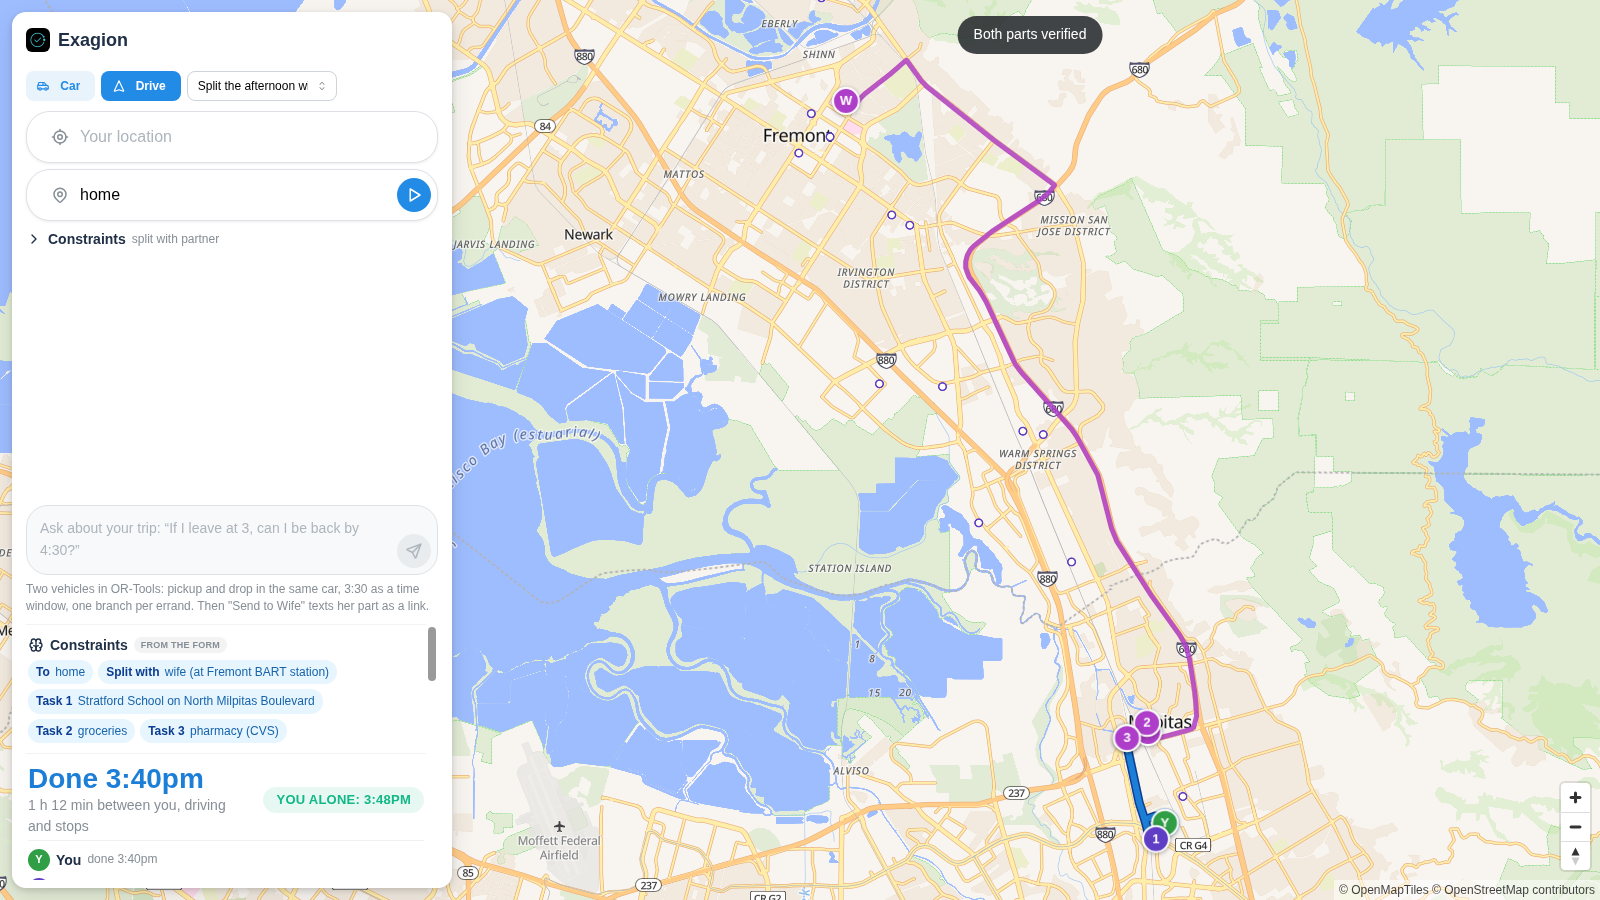
\includegraphics[height=0.65\textheight,keepaspectratio,trim=452 0 0 0,clip]{gm-team.png}
    \end{column}
  \end{columns}
\end{frame}

\begin{frame}{Sending a driver their part}
  \begin{columns}[T]
    \begin{column}{0.66\textwidth}
      \begin{itemize}
        \item ``Send to Wife'': a link with an unguessable token, valid 30 minutes; no account, no app
        \item The page shows her part of the plan and can share her location back
        \item ``Start turn-by-turn'': Ferrostar in her browser, on the plan's exact route request (exclusions kept on reroute)
        \item On expiry the position is deleted and the link returns 410
        \item Limits: browsers share location only while the page is open; Google Maps location sharing has no API
      \end{itemize}
    \end{column}
    \begin{column}{0.26\textwidth}
      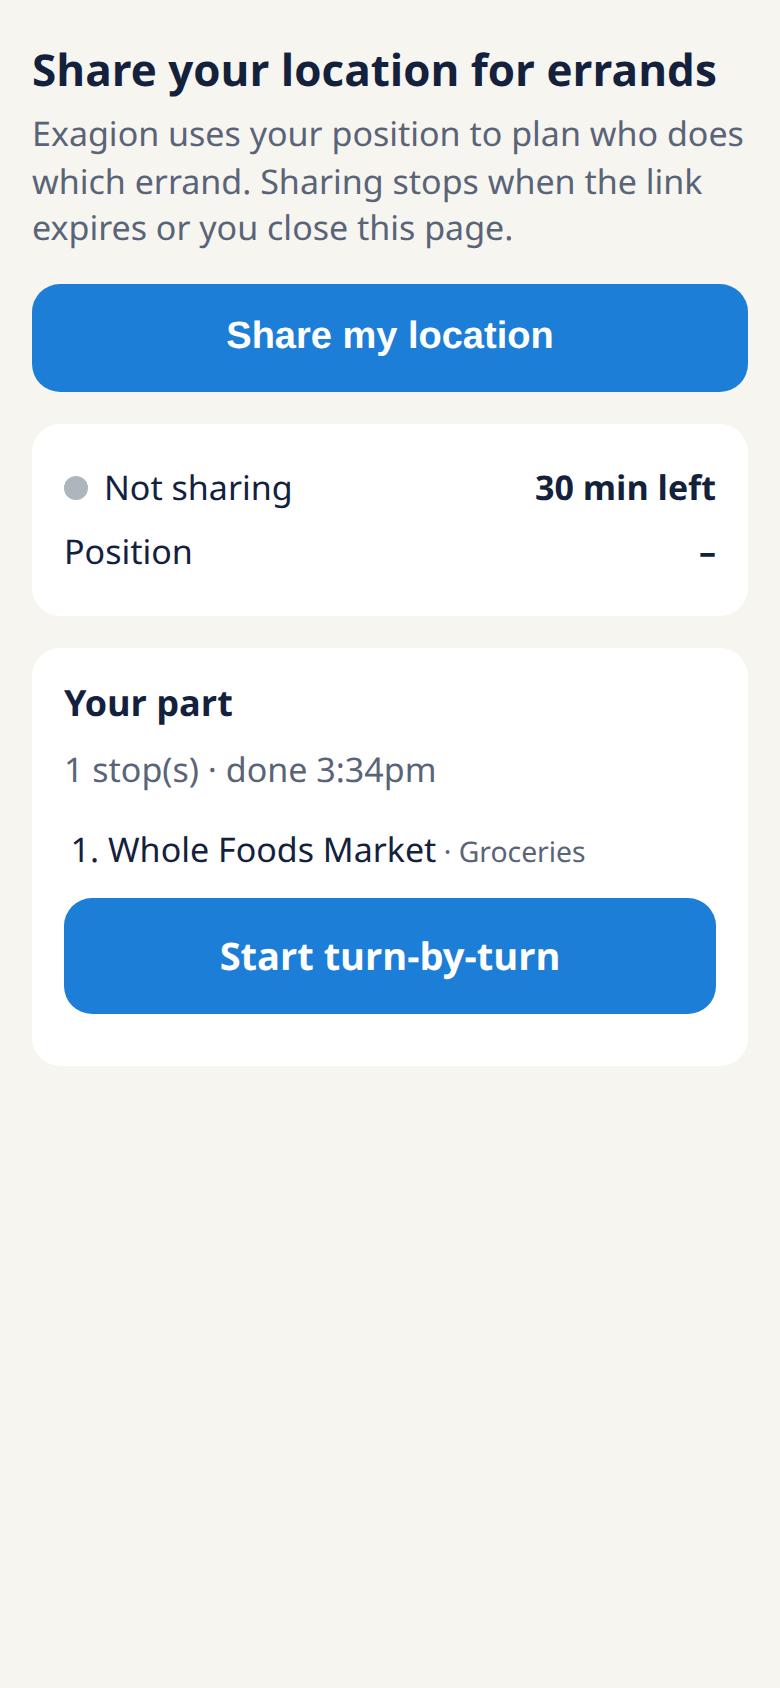
\includegraphics[height=0.78\textheight,keepaspectratio]{gm-team-phone.png}
    \end{column}
  \end{columns}
\end{frame}

% ------------------------------------------------------------------------------------------------
\section{Verification}

\begin{frame}{Every route is checked independently of the planner}
  \begin{itemize}
    \item The final line is map-matched again (\api{/trace\_attributes}); checks read those edges, not the planner's state
    \item Checked: stops reached and in order; roads and areas avoided; detour bounds; side of road on arrival; ``about $N$ min in''; closing times; deadline; pickup before drop in the same car
    \item A failed check is shown with the measured value; the route is still drawn
    \item Retry loops fix loud failures; the verifier makes silent failures loud
    \item Silent failures seen in practice: an exclusion polygon rejected by the engine, a stop skipped by the solver, a deadline missed by a relaxed solve
  \end{itemize}
\end{frame}

% ------------------------------------------------------------------------------------------------
\section{Where it breaks}

\begin{frame}{Data: the verifier cannot catch a wrong category}
  \begin{itemize}
    \item Overture places with confident, wrong categories:
      \begin{itemize}
        \item Oportun ($\approx$20 sites): pharmacy; a lender (confidence 0.92--0.99)
        \item Evernote: gas station; Biocardia: pharmacy
        \item Hills Bros.\ Coffee Plant: coffee shop; a historic building
        \item Gano Excel (Fairfield): coffee shop; a coffee company's business-park unit
      \end{itemize}
    \item The route does stop where the data says a pharmacy is: geometric checks pass
    \item Mitigation: a small, visible deny list in code; better: report upstream
    \item Geocoding ranks names, not meaning: ``Oakland airport'' $\to$ Oakland Airport Executive Hotel, until the OSM tag had to match the named kind
  \end{itemize}
\end{frame}

\begin{frame}{Engines: silent failures}
  \begin{itemize}
    \item Valhalla matrices: $\approx$2\% of places null in their entire row and column (8 of 400 shops); all snapped to a parking aisle or service road; \api{/route} reaches them. Fix: re-snap those points to the street
    \item Default \api{max\_exclude\_polygons\_length}: 10 km total perimeter; over it the request is rejected, and the easy fallback silently drops the constraint
    \item Ollama: tool-call arguments must be objects, not JSON strings; every turn after a tool call failed
    \item Ollama: two context sizes (8k, 16k) load two copies of a 35B model; on a 12 GB GPU the second load crashed
  \end{itemize}
\end{frame}

\begin{frame}{Impossible requests: say no, with the number}
  \begin{columns}[T]
    \begin{column}{0.38\textwidth}
      \begin{itemize}
        \item ``Home by five'' at 4:55 with three errands: OR-Tools relaxes the deadline; the verifier fails it: arrive 5:05
        \item ``A car wash under one minute out of the way'': the closest adds 3.2 min
        \item Never a plausible route that quietly violates the request
      \end{itemize}
    \end{column}
    \begin{column}{0.6\textwidth}
      \shot{breaks-deadline.png}
    \end{column}
  \end{columns}
\end{frame}

\begin{frame}{What constraints cannot express yet}
  \begin{itemize}
    \item ``Downtown'': no usable boundary in OSM; a gazetteer circle
    \item ``The Bay Bridge'': the name is in \texttt{bridge:name}, absent from the routing graph; matched by footprint for a short list
    \item ``Before it closes'': no opening hours in the open places data; the driver must state the time
    \item ``A Safeway'': resolution picks one; alternatives are shown, not asked
    \item A verifier that shares the planner's definitions shares its mistakes: checks need independent data, not only independent code
  \end{itemize}
\end{frame}

% ------------------------------------------------------------------------------------------------
\section{Conclusion}

\begin{frame}{Summary}
  \begin{enumerate}
    \item Give the language model one job: fill a typed schema. Open engines do the geometry and the optimization.
    \item Constraints are predicates over graph edges, not road names; iterate until the route satisfies them.
    \item Verify the final route from fresh data, and report failures with the measured value.
  \end{enumerate}
\end{frame}

\begin{frame}{Thank you}
  \begin{itemize}
    \item Code: github.com/johngcarlsson-usc/TurnByTurn
    \item Built on Valhalla, OpenStreetMap, Overture Maps, DuckDB, OR-Tools, Photon, Nominatim, Caltrans PeMS, Ferrostar, MapLibre, OpenFreeMap, Open-Meteo, Ollama
  \end{itemize}
\end{frame}

\end{document}
